% JUMP TO LINE 60, 75
\documentclass[preview, margin=0.6in]{standalone}
\usepackage[letterpaper,portrait,top=0.4in, left=0.6in, right=0.6in, bottom=1in]{geometry}

\usepackage{amsmath, amsfonts, amsthm, amssymb}
\usepackage{graphicx, float}
\usepackage{mathtools}
\usepackage{titlesec}
\usepackage{interval}
\usepackage{hyperref}
\usepackage{siunitx}
\usepackage{titling}
\usepackage{vwcol}
\usepackage{setspace}
\usepackage{empheq}
\usepackage{cancel}
\usepackage{esdiff}
\usepackage{multicol}
\usepackage{mdframed}
\usepackage{esdiff}
\usepackage{tikzsymbols}
\usepackage{multicol}
\usepackage{tikz}
\usepackage{varwidth}
\usepackage{parskip}
\usepackage{pgfplots}
\usepackage{mlmodern}
\pgfplotsset{compat=1.18}
\intervalconfig {
	soft open fences
}

\newcommand{\alignedintertext}[1]{%
  \noalign{%
    \vtop{\hsize=\linewidth#1\par
    \expandafter}%
    \expandafter\prevdepth\the\prevdepth
  }%
}

\newtheorem{lemma}{Lemma}

\newcommand*{\problem}[1]{\section*{Problem #1}}
\newcommand*{\aps}{\section*{AP Corner}}
\newcommand*{\deriv}[1][x]{\ensuremath{\dfrac{\mathrm{d}}{\mathrm{d}#1}}}
\newcommand*{\floor}[1]{\ensuremath{\lfloor #1\rfloor}}
\newcommand*{\lheqzero}{\ensuremath{\underset{\text{L'H}}{\overset{\left[\frac00\right]}{=}}}}
\newcommand*{\lheqinfty}{\ensuremath{\underset{\text{L'H}}{\overset{\left[\frac{\infty}{\infty}\right]}{=}}}}

\DeclareMathOperator{\DNE}{DNE}
\DeclareMathOperator{\sgn}{sgn}

\DeclareMathOperator{\arccsc}{arccsc}
\DeclareMathOperator{\arcsec}{arcsec}
\DeclareMathOperator{\arccot}{arccot}

%opening

\title{\vspace*{-40pt}Homework Set 3C}
\author{Jayden Li}
\date{\today}
% \allowdisplaybreaks
\postdisplaypenalty=100000

\begin{document}
\setstretch{1.25}
\fontsize{12pt}{12pt}\selectfont
\setlength{\abovedisplayskip}{\abovedisplayskip/2}
\setlength{\belowdisplayskip}{\belowdisplayskip/2}
\setlength{\parindent}{0pt}
\setlength{\parskip}{2ex plus 0.5ex minus 0.2ex}
\maketitle

\problem{1}
Any point $(x,y,z)$ on the line is a scalar multiple of the vector $v=(1,-2,3)$:
\begin{equation*}
	(x,y,z)
	=av
	=(a,-2a,3a)
	\iff \left\{ 
		\begin{aligned}
			x&=a \\
			y&=-2a=-2x \\
			z&=3a=3x
		\end{aligned}
	\right.
\end{equation*}
A point is on the line if and only if we can write it in the form $(x,-2x,3x)$, where $x\in\mathbb R$.
\begin{center}
	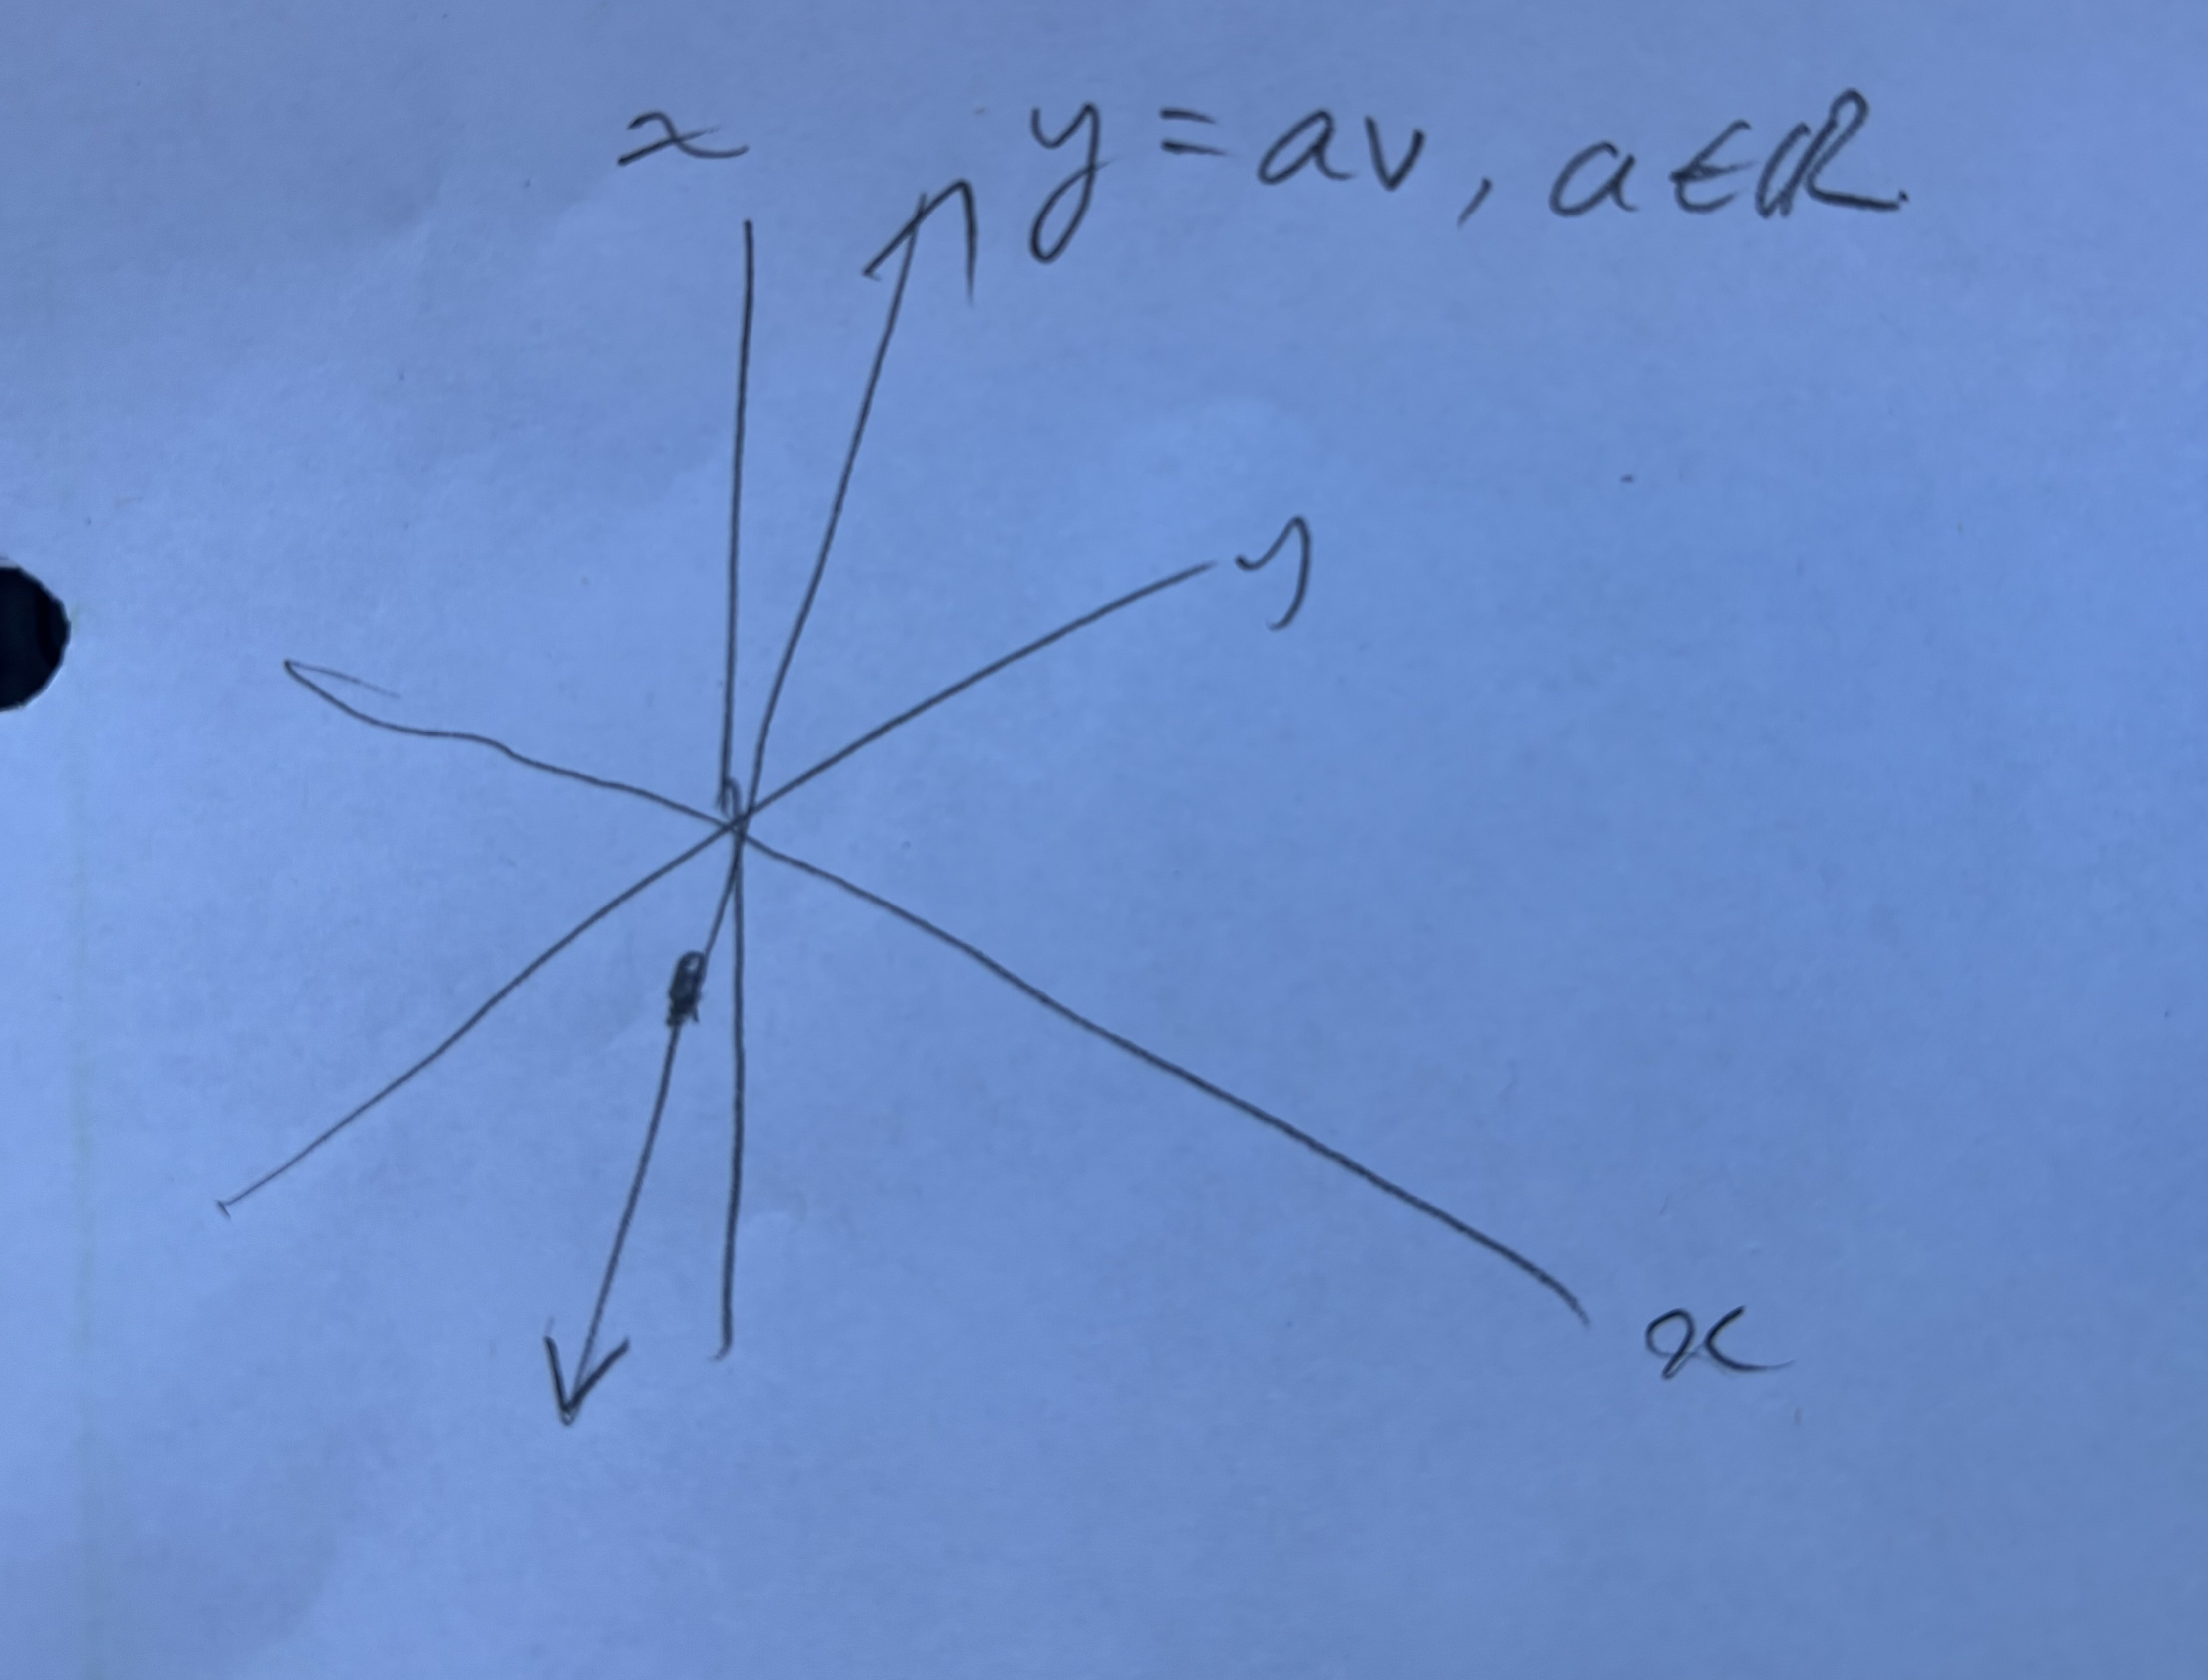
\includegraphics[width=0.5\linewidth]{IMG_5524.jpeg}
\end{center}

\problem{2}
Any satisfying the equation $y=2x$ can be written as $(a curve or other figure formed by all the points satisfying a particular equation of the relation between coordinates, or by a point, line, or surface moving according to mathematically defined conditions.x,2x,z)$, where $x,z\in\mathbb R$. Since there are 2 free variables, the set of points satisfying the equation is a plane.
\begin{center}
	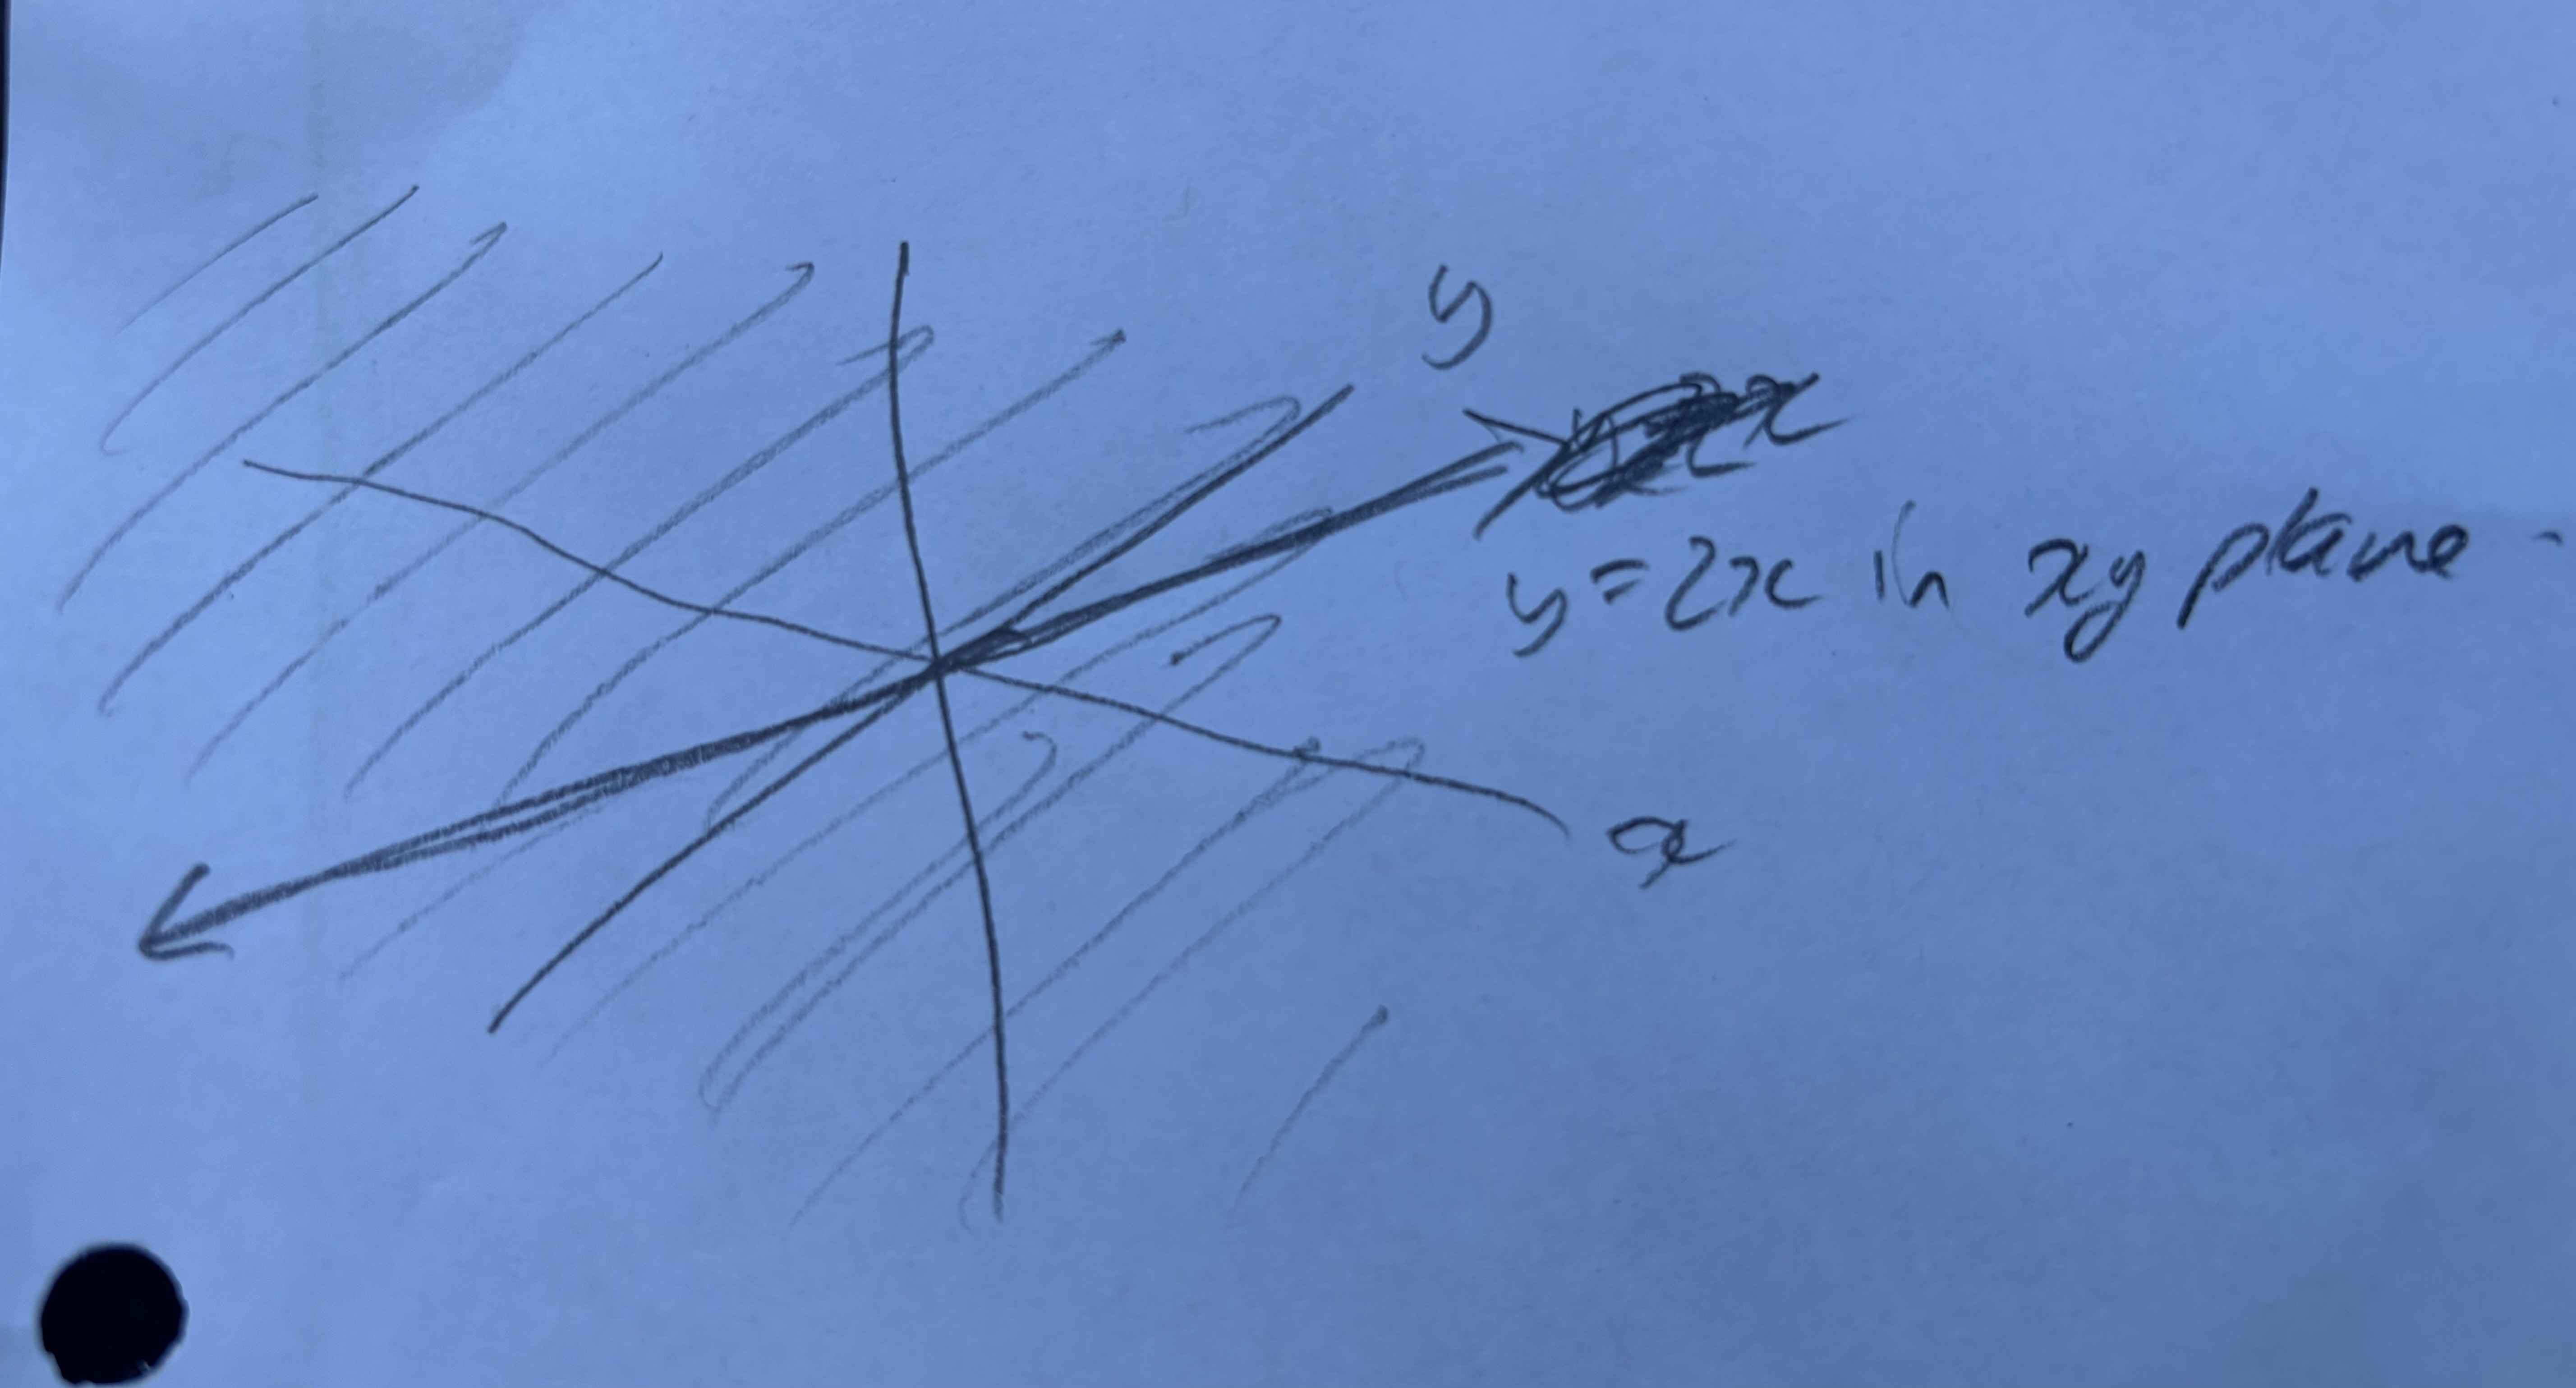
\includegraphics[width=0.5\linewidth]{IMG_5525.jpeg}
\end{center}

\end{document}
